% !TEX root=./../maha-dip-notes.tex
\section{Linear System or Filters}

Linear systems and their associated filters form the foundation for many image processing techniques. Filters are algorithms or operations that modify pixel values based on defined rules, often employing local neighborhoods.

\paragraph{Consider a system \( T \) that processes images (signals).}

Suppose we apply the system \( T \) to two different input images \( f_1 \) and \( f_2 \)
\[
T(f_1) = g_1, \quad T(f_2) = g_2
\]
where \( g_1 \) and \( g_2 \) are the corresponding output images.

\subsection{Linearity}
The system \( T \) is \textbf{linear} if it satisfies both additivity and homogeneity, 
\begin{align*}
T(f_1 + f_2) &= T(f_1) + T(f_2) &= g_1 + g_2 \qquad \qquad &\text{(additivity)} \\
T(a f_1) &= a T(f_1) &= a g_1  \qquad \qquad \qquad  &\text{(homogeneity)} 
\end{align*}
or equivalently, it satisfies the property of \textit{superposition},
\[
T(a f_1 + b f_2) = a T(f_1) + b T(f_2) = a g_1 + b g_2
\]
for any constants \( a, b \).

This means the system's response to a weighted sum of inputs is the weighted sum of the responses.

\dfn{Linear Filter}{A filter or system is \emph{linear} if it obeys both additivity and homogeneity, that is, for any images $f$ and $g$, and scalars $a$ and $b$, the response $\mathcal{F}$ satisfies $$\mathcal{F}[a f + b g] = a \mathcal{F}[f] + b \mathcal{F}[g]$$.}

\subsection{Shift (Translation) Invariance}

The system \( T \) is \textbf{shift invariant} if shifting the input image results in a corresponding shift in the output, If we shift \( f \) by \((x_0,y_0)\),
\[
f'(x,y) = f(x - x_0, y - y_0),
\]
then the output shifts by the same amount:

\[
T(f') = g'(x,y) = g(x - x_0, y - y_0).
\]
The system behaves the same regardless of where the input pattern is located.


\dfn{Shift Invariance}{
If $\mathcal{F}$ is a shift-invariant system, then for any image $f(x,y)$ and shift $(x_0, y_0)$:
$$
\mathcal{F}[f(x-x_0, y-y_0)] = [\mathcal{F}[f(x,y)]]_{(x-x_0, y-y_0)}
$$
}

\subsection{Impulse (Delta) Function}
\dfn{Impulse (Delta) Function}{
The \textbf{impulse} or \textbf{Dirac delta function} \( \delta(x,y) \), defined as

\[
\delta(x, y) = \begin{cases}
\infty, & x=0, y=0 \\
0, & \text{elsewhere}
\end{cases}
\quad \text{and} \quad \int_{-\infty}^{\infty}\int_{-\infty}^{\infty} \delta(x,y) dx dy = 1
\]
}
\noindent \textbf{Pictorial representation of a 1D continuous dirac delta function}
% Continuous impulse function (Dirac delta)
\begin{center}
    \begin{tikzpicture}[scale=2]
        % Axes
        \draw[->] (-0.5,0) -- (2,0) node[right] {$x$};
        \draw[->] (0,-0.5) -- (0,2.5) node[above] {$\delta(x)$};
        
        % Impulse
        \draw[line width=2pt] (0,0) -- (0,2);
        \node[above] at (-0.1,2.1) {$\infty$};
        
        % Label
        \draw[dashed] (0,-0.1) -- (0,0);
        \node[below] at (-0.1,-0.1) {0};
        
        % Integral annotation
        \node[right] at (0.3,1.2) {\small $\int_{-\infty}^\infty \delta(x)dx = 1$};
    \end{tikzpicture}
\end{center}
The impulse acts like an identity element to "probe" the system.


\dfn{Discrete Impulse}{The \emph{discrete impulse} $\delta(x, y)$ is defined as
$$
\delta(x, y) = 
\begin{cases}
1 & \text{if } x = 0,~y = 0 \\
0 & \text{otherwise}
\end{cases}
\quad \text{and} \quad \sum_{x =-\infty}^{\infty}\sum_{y = -\infty}^{\infty} \delta(x,y) = 1.
$$
}

\noindent \textbf{Pictorial representation of a 1D discrete dirac delta function}
% Discrete impulse function with width epsilon
\begin{center}
    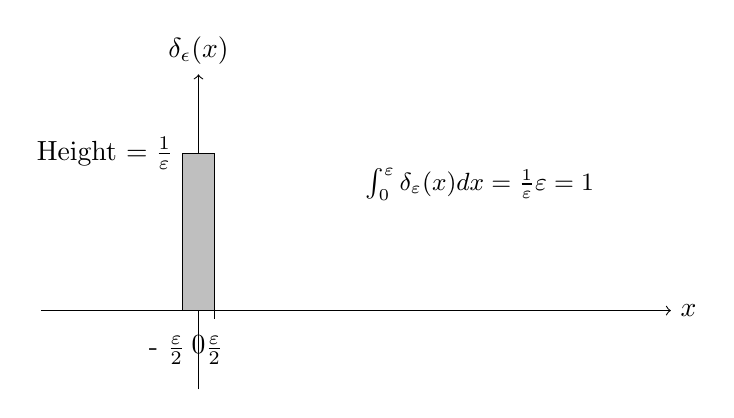
\begin{tikzpicture}[scale=2]
        % Axes
        \draw[->] (-1,0) -- (3,0) node[right] {$x$};
        \draw[->] (0,-0.5) -- (0,1.5) node[above] {$\delta_\epsilon(x)$};

        % Rectangle for impulse of width epsilon
        \def\eps{0.1}
        \draw[fill=gray!50] (-\eps,0) rectangle (\eps,1);

        % Base line
        \draw (0,0) -- (\eps,0);

        % Labels
        \draw[dashed] (0,0) -- (0,-0.1);
        \draw[dashed] (\eps,0) -- (\eps,-0.1);

        \node[below] at (0,-0.1) {0};
        \node[below] at (\eps,-0.1) {$\frac{\varepsilon}{2}$};
        \node[below] at (-2*\eps,-0.1) { - $\frac{\varepsilon}{2}$};
        \node[left] at (- \eps,1) {Height $= \frac{1}{\varepsilon}$};

        % Integral annotation
        \node[right] at (1,0.8) {\small $\int_{0}^{\varepsilon} \delta_\varepsilon(x) dx = \frac{1}{\varepsilon} \varepsilon = 1$};
    \end{tikzpicture}
\end{center}

In discrete images, \( \delta[x,y] \) equals 1 at \((0,0)\) and 0 elsewhere.

\subsection{Linear and Shift-Invariant (LSI) Systems}
A system that is both linear and shift-invariant is known as an \textbf{LSIS}. For inputs $f_1$ and $f_2$ and outputs \( g_1 \) and \( g_2 \), and a scalar \( \alpha \), the following properties must hold

\begin{align*}
T(\alpha f_1 + f_2) &= \alpha T(f_1) + T(f_2) \\
T(f(x,y)) &= T(f(x-a,y-b))
\end{align*}  

we can think of linearity as a superposition of weighted impulse responses, and shift-invariance as the ability to shift the input and output without changing the system's behavior. for example, linearity in brightness variation and shift invariance is scene movement.

These systems can be completely characterized by their response to a single, special input called the {\it impulse function}.

\subsection{Convolution}
Given an input \( f(x,y) \), it can be represented as an integral over shifted impulses weighted by the value of \( f \)

\[
f(x,y) = \int_{-\infty}^\infty \int_{-\infty}^\infty f(\xi, \eta) \, \delta(x-\xi, y-\eta) \, d\xi d\eta.
\]
Applying \( T \) and using linearity:
\[
g(x,y) = T(f)(x,y) = \int_{-\infty}^\infty \int_{-\infty}^\infty f(\xi,\eta) T(\delta(x-\xi, y-\eta)) \, d\xi d\eta.
\]
Using shift invariance:
\[
T(\delta(x-\xi, y-\eta)) = h(x-\xi, y-\eta).
\]
Therefore,
\[
g(x,y) = \int_{-\infty}^\infty \int_{-\infty}^\infty f(\xi,\eta) h(x-\xi, y-\eta) \, d\xi d\eta = (f * h)(x,y).
\]
This integral is known as the \textit{convolution} of \( f \) with \( h \).


\dfn{Convolution}{
Convolution of two functions $f$ and $h$ is defined as
\[
    g(x)  = f(x) \textasteriskcentered h(x) = \int_{-\infty}^{\infty} f(\tau) h(x - \tau) d\tau
\]

for two dimensions we have 

\[ 
    g(x,y) = f(x, y) \textasteriskcentered h(x, y) = \int_{-\infty}^{\infty} \int_{-\infty}^{\infty} f(\tau_1, \tau_2) h(x - \tau_1, y - \tau) d\tau_1 d\tau_2
\]
}

\paragraph{Intution of convolution.} Convolution is a mathematical operation that combines two functions to produce a third function that expresses how the shape of one is modified by the other. we call the $h(x)$ function as kernel, which is used to modify the shape of the other function.
\begin{itemize}
    \item $- \tau$ says that we need to flip the kernel (in x-axis)
    \item $h(x - \tau)$ says that we iterate over all $\tau$'s with the fliped kernel (in x-axis)
    \item The kernel is applied to the signal $f(x)$ by sliding it over the $\tau$ for all values and computing the dot product of the kernel and the function at each position. 
    \item The result of the dot product is the value of the new signal $(g(x))$ at that position.
    \item This new signal $g(x)$ is the convolution.
\end{itemize}

\nt{
    Best youtube videos on this topic, worth watching to get an intution visually 
    \begin{itemize}
        \item \href{https://youtu.be/0OHRJMNKhX0}{LSIS and Convolution | Image Processing I} by Shree Nayar
        \item \href{https://youtu.be/KuXjwB4LzSA}{But what is a convolution?} by 3Blue1Brown
    \end{itemize}   
}

\dfn{Discrete spatial Convolution}{
Discrete spatial convolution is defined as
\[ 
    g(x) = f(x) \textasteriskcentered h(x) = \sum_{\tau} f(\tau) h(x - \tau)
\]
            
for two dimensions, the convolution of an image $f(x, y)$ and kernel $h(i, j)$ is defined as:
$$
g(x) = (f \textasteriskcentered h)(x, y) = \sum_{i} \sum_{j} f(x - i, y - j) h(i, j)
$$
}

\paragraph{Properties of Convolution}
\begin{itemize}
    \item \textbf{Commutative}: $f * h = h * f$
    \item \textbf{Associative}: $(f * h) * g = f * (h * g)$
    \item \textbf{Distributive}: $f * (h + g) = f * h + f * g$
\end{itemize}
\nt{Convolution is the central operation for applying filters to images, especially linear spatial filters.}


\ex{Convolution example of two uniformly distributed signals}{
Consider two functions \(f\) and \(h\) defined as uniform distributions on the interval \([-1,1]\)

\[
f(x) = h(x) = U(-1,1) = \begin{cases}
1, & x \in [-1,1], \\
0, & \text{otherwise}.
\end{cases}
\]

The convolution \(g = f * h\) is given by
\[
    g(x) = (f*h)(x) = \int_{-\infty}^{\infty} f(\tau) h(x-\tau)\, d\tau.
\]

\textbf{Overlap analysis}\\
\begin{itemize}
    \item For $|x| \geq 2$, no overlap, so $g(x) = 0$.  
    \item For $-2 \leq t \leq 0$, the overlap length grows linearly: $g(x) = x + 2$.  
    \item For $0 \leq t \leq 2$, the overlap length decreases linearly: $g(x) = 2 - x$.  
\end{itemize}

\textbf{Final Result}\\
Thus,
\[
g(x) =
\begin{cases}
0 & |x| \geq 2, \\[6pt]
x+2 & -2 \leq x < 0, \\[6pt]
2-x & 0 \leq x \leq 2.
\end{cases}
\]

Since both \(f\) and \(h\) are uniform rectangles, their convolution \(g(x)\) is a \textbf{triangle function} defined as

\[
g(x) = \begin{cases}
0, & |x| \ge 2, \\
(2 - |x|), & |x| < 2.
\end{cases}
\]
with base $[-2,2]$ and peak value $2$ at $t=0$.

\textbf{Illustration}\\
\begin{center}
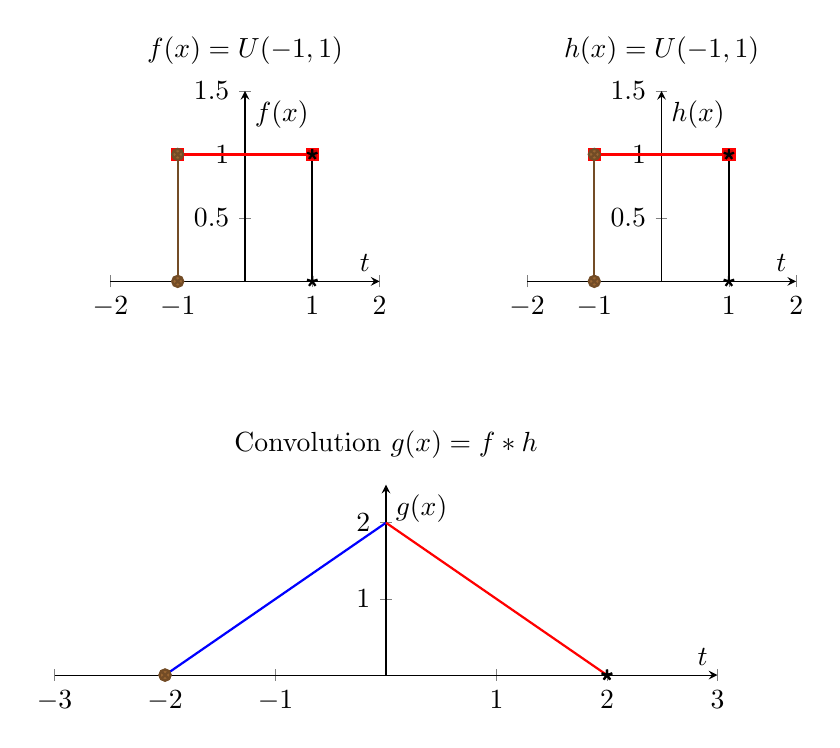
\begin{tikzpicture}[scale=1.0]
% f(x)
\begin{axis}[width=5cm, height=4cm, xlabel={$t$}, ylabel={$f(x)$}, title={$f(x) = U(-1,1)$}, axis lines=middle, ymin=0, ymax=1.5, xmin=-2, xmax=2]
\addplot+[ycomb, mark=none, thick] coordinates {(-1,1) (1,1)};
\addplot+[thick] coordinates {(-1,1) (1,1)};
\addplot+[thick] coordinates {(-1,0) (-1,1)};
\addplot+[thick] coordinates {(1,0) (1,1)};
\end{axis}

% h(x)
\begin{axis}[at={(7cm,0)}, anchor=origin, width=5cm, height=4cm, xlabel={$t$}, ylabel={$h(x)$}, title={$h(x) = U(-1,1)$}, axis lines=middle, ymin=0, ymax=1.5, xmin=-2, xmax=2]
\addplot+[ycomb, mark=none, thick] coordinates {(-1,1) (1,1)};
\addplot+[thick] coordinates {(-1,1) (1,1)};
\addplot+[thick] coordinates {(-1,0) (-1,1)};
\addplot+[thick] coordinates {(1,0) (1,1)};
\end{axis}

% g(x)
\begin{axis}[at={(3.5cm,-5cm)}, anchor=origin, width=10cm, height=4cm, xlabel={$t$}, ylabel={$g(x)$}, title={Convolution $g(x) = f*h$}, axis lines=middle, ymin=0, ymax=2.5, xmin=-3, xmax=3]
\addplot+[thick, mark=none, domain=-2:0, samples=100] {x+2};
\addplot+[thick, mark=none, domain=0:2, samples=100] {2-x};
\addplot+[thick] coordinates {(-2,0) (-2,0)};
\addplot+[thick] coordinates {(2,0) (2,0)};
\end{axis}
\end{tikzpicture}
\end{center}
\noindent
The above graph shows the input functions \(f\) and \(h\) (both uniform rectangles). The below graph shows their convolution \(g\), a triangle with base length 4 and height 2.
}

\paragraph{Convolution is linear.} Convolution is linear, which means that for any functions \(f_1\), \(g_1\), \(f_2\), \(g_2\), and \(h\), and any constants \(a\) and \(b\), if 
\[
    g_1(x) = (f_1*h)(x) = \int_{-\infty}^{\infty} f_1(t)h(x-t)dt \quad \text{and} \quad g_2(x) = (f_2*h)(x) = \int_{-\infty}^{\infty} f_2(t)h(x-t)dt
\]
Then, 
\begin{align*}
    ((a f_1 + b f_2) * h )(x) &= \int_{-\infty}^{\infty} (a f_1 + b f_2)(t)h(x-t)dt\\
    &= a \int_{-\infty}^{\infty} f_1(t)h(x-t)dt  + b \int_{-\infty}^{\infty}  f_2(t)h(x-t)dt\\
    &= a g_1(x) + b g_2(x)
\end{align*}


\paragraph{Convolution is Shift invariant.} Convolution is shift invariant, which means that for any functions \(f\), \(g\), and \(h\),and any constants \(a\), if 
\[
    g(x) = (f*h)(x) = \int_{-\infty}^{\infty} f(t)h(x-t)dt
\]
Then, 
\begin{align*}
    \int_{-\infty}^{\infty} f(t - a )h(x-t)dt &= \int_{-\infty}^{\infty} f(\mu)h(x - \mu - a)dt \qquad \qquad \text{using }\; \mu = t - a\\ 
    &= \int_{-\infty}^{\infty} f(\mu)h((x - \mu) - a)dt\\ 
    &= g(x - a)
\end{align*}
Hence, {\bf Convolution is a linear shift invariant system (LSIS)}.

\subsubsection{Finding the Filter $h$}
Given the convolution system with $h(x)$ hidden, How can we find it?

\noindent {\bf Yes}, We can use the function $f(x)$ as a unit impulse function. As the \emph{discrete impulse} $\delta(x, y)$ is defined as
$$
\delta(x, y) = 
\begin{cases}
1 & \text{if } x = 0,~y = 0 \\
0 & \text{otherwise}
\end{cases}
\quad \text{and} \quad \sum_{x =-\infty}^{\infty}\sum_{y = -\infty}^{\infty} \delta(x,y) = 1.
$$

\paragraph{Sifting property}When we convolve any function $f(x)$ with $\delta$ then the resulting function is $f(x)$ itself, acting as a identity operation, also known as sifting property. 
\[
    g(x) = (\delta*h)(x) = \int_{-\infty}^{\infty} \delta(t)h(x-t)dt = h(x)
\]
similarly,
\[
    g(x) = (f*\delta)(x) = \int_{-\infty}^{\infty} f(t)\delta(x-t)dt = f(x)
\]
This shows that convolving with \(\delta\) leaves the signal unchanged.

\paragraph{Proof:}
Starting with the convolution definition,
\[
(f * \delta)(x) = \int_{-\infty}^\infty f(t) \delta(x - t) dt,
\]
the delta function \(\delta(x - t)\) is zero everywhere except at \(t = x\), where it is infinite with unit integral. Thus the integral "picks out" the value \(f(x)\):
\[
(f * \delta)(x) = f(x).
\]

\subsection{Correlation}

\dfn{Correlation}{Discrete correlation for image $f(x, y)$ and kernel $h(i, j)$ is:
$$
    (f \circ h)(x, y) = \sum_{i} \sum_{j} f(x + i, y + j) h(i, j)
$$
}

\paragraph{Effect of Dirac Impulse on Correlation}

Applying correlation with the discrete impulse \(\delta\),
\[
(\delta \circ h)(x) = \sum_{i} f(x+i) \, \delta(i).
\]
By definition of \(\delta(i)\), the only nonzero term is at \(i = 0\), so
\[
(\delta \circ h )(x) = h(-x).
\]
Thus, correlation with the Dirac impulse also acts as an identity, leaving the image unchanged.

\paragraph{Relation of Convolution and Correlation}
Convolution involves a kernel flip (i.e., $h(-i, -j)$), while correlation does not. For symmetric kernels, convolution and correlation produce identical results.

\clm{Equivalence for Symmetric Kernels}{}{
If $h(i, j)$ is symmetric ($h(i, j) = h(-i, -j)$), then convolution and correlation yield the same output.
}
\nt{Many image processing kernels (e.g., Gaussian blur) are symmetric, so the distinction between convolution and correlation may disappear in practical settings.}
